\subsection{Development process}

\subsubsection{SCRUM model}
	
The most used model for iterative, incremental development of the projects these
days is SCRUM. It is an agile software development strategy which uses iterative 
development as a basis, but advocates a lighter and more people-centric viewpoint
than traditional approaches. Agile processes use feedback, rather than planning
as their primary control mechanism. The feedback is driven by regular tests and
releases of the evolving software. \cite{wiki:development-process}\newline
	
Although the Scrum approach was originally suggested for managing product development
projects, its use has focused on the management of software development projects, 
and it can be used to run software maintenance teams or as a general 
project/program management approach.\newline
	
Scrum is a process skeleton that contains sets of practices and predefined roles.
The main roles in Scrum are:
	
\begin{itemize}
	\item the ScrumMaster, who maintains the processes (typically in lieu of a project manager)
	\item the Product Owner, who represents the stakeholders and the business
	\item the Team, a cross-functional group who do the actual analysis, design, implementation, testing, etc.
\end{itemize}

\begin{figure}[htb]
	\centering
	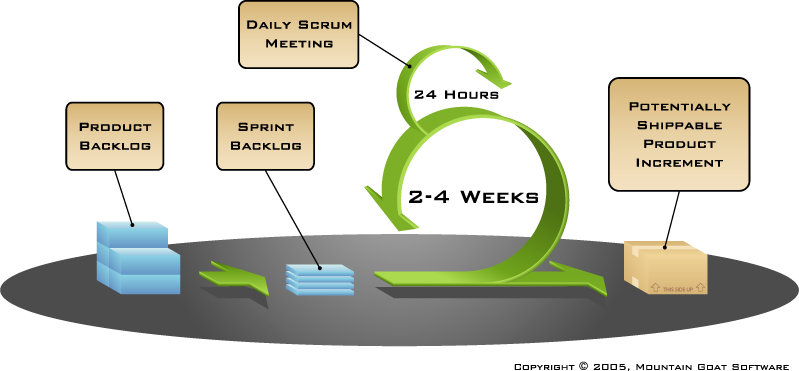
\includegraphics[width=0.8\textwidth]{process/development_process/scrum.png}
	\caption{Scrum methodology\cite{targetprocess:scrum}}
	\label{fig:scrum-methology}
\end{figure}

During each sprint, typically a two to four week period (with the length decided by the team), 
the team creates a potentially deliverable product each increment. 
The set of features that go into a sprint come from the product backlog, 
which is a prioritized set of high level requirements of work to be done. 
Which backlog items go into the sprint is determined during the sprint planning meeting. 
During this meeting, the Product Owner informs the team of the items in the product backlog that he 
or she wants completed. 
The team then determines how much of this they can commit to complete during the next sprint, 
and records this in the sprint backlog. 
During a sprint, no one is allowed to change the sprint backlog, which means that the requirements
are frozen for that sprint. Development is timeboxed such that the sprint must end on time. 
If requirements are not completed for any reason they are left out and returned to the product backlog. 
After a sprint is completed, the team demonstrates how to use the software.

Scrum enables the creation of self-organizing teams by encouraging verbal communication between all team members situated at one location.

A key principle of Scrum is its recognition that during a project the customer can change their
mind about what they want and need, and that unpredicted challenges cannot be easily addressed 
in a traditional predictive or planned manner. 
As such, Scrum adopts an empirical approach, accepting that the problem cannot be fully understood 
or defined at the start, focusing instead on maximizing the team’s ability to deliver quickly and
respond to new requirements.

\subsubsection{Waterfall model}
The waterfall model is a sequential design process, often used in software development processes, 
in which progress is seen as flowing steadily downwards (like a waterfall) through the phases of
Conception, Initiation, Analysis, Design, Construction, Testing, Production/Implementation and Maintenance.

\begin{figure}[htb]
	\centering
	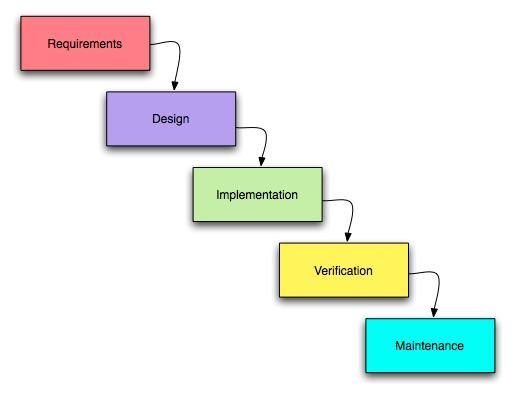
\includegraphics[width=0.8\textwidth]{process/development_process/waterfall.jpg}
	\caption{The unmodified "waterfall model" methodology\cite{worldpress:waterfall}}
	\label{fig:waterfall-model}
\end{figure}

In Royce's original waterfall model, the following phases are followed in order:

\begin{itemize}
	\item Requirements specification
	\item Design
	\item Construction (AKA implementation or coding) testing, etc.
	\item Integration
	\item Testing and debugging (AKA Validation)
	\item Installation
	\item Maintenance
\end{itemize}

Thus the waterfall model maintains that one should move to a phase only when its preceding phase is 
completed and perfected. However, there are various modified waterfall models (including Royce's final model) 
that may include slight or major variations upon this process.\newline\newline

\subsubsection{Conclusion}
For this project, the team decided to use the SCRUM model. But as SCRUM requires strict and precise
execution of the predefined model, the actual development process will be slightly modified. 
The project will have 4 sprints, including additional an 'zero' sprint which contained the initial
prestudy and GUI sample. Each sprint will span 2 weeks, or 10 working days. 
Some additional time will be left after completition of the sprints for revision, 
fixing and more testing, to improve the product's reliability and quality if necessary.
